\newpage
\section{Project Management with Scrum}

This section outlines the key aspects of project management with Scrum including the product backlog, use case diagram, sprint planning, and interface prototyping.

\subsection{Backlog Features}

\begin{longtable}{|c|p{0.83\textwidth}|c|}
	\hline
	\textbf{ID} & \textbf{Description} & \textbf{Effort} \\
	\hline
	1           & Register for an account with a password and email to access the system. & Low \\
	\hline
	2           & Log in to the account using email and password for secure access. & Low \\
	\hline
	3           & Reset the password via email in case of forgetting it. & Low \\
	\hline
	4           & Create a new organization with a unique name and become its administrator to manage users and templates. & High \\
	\hline
	5           & View a list of all organizations to navigate and manage them. & Medium \\
	\hline
	6           & Access shared work (templates, campaigns, media) within the organization for effective collaboration. & High \\
	\hline
	7           & Deactivate or remove users from the organization for security and access control. & Medium \\
	\hline
	8           & Add users to the organization and assign specific roles for access control. & High \\
	\hline
	9           & View and manage user roles within the organization. & Medium \\
	\hline
	10          & Create new email templates for sending emails. & High \\
	\hline
	11          & Edit and update email templates to keep information accurate. & Medium \\
	\hline
	12          & View a list of all email templates for easy management. & Low \\
	\hline
	13          & Create and manage email template drafts before finalizing and sending. & High \\
	\hline
	14          & Create and publish campaigns using selected templates to organize and track marketing efforts.. & High \\
	\hline
	15          & View a history of published campaigns for reference. & Low \\
	\hline
	16          & Generate reports for campaign analysis and informed decision-making. & High \\
	\hline
\end{longtable}

\clearpage
\subsection{Global Use Case Diagram}
Figure \ref{fig:Global Use Case Diagram} offer us a global overview by presenting a visual description of the functional
behaviour of our tool. This diagram sums up the interactions among the actors and the
diverse use cases within the system.

\begin{figure}[ht]
	\centering
	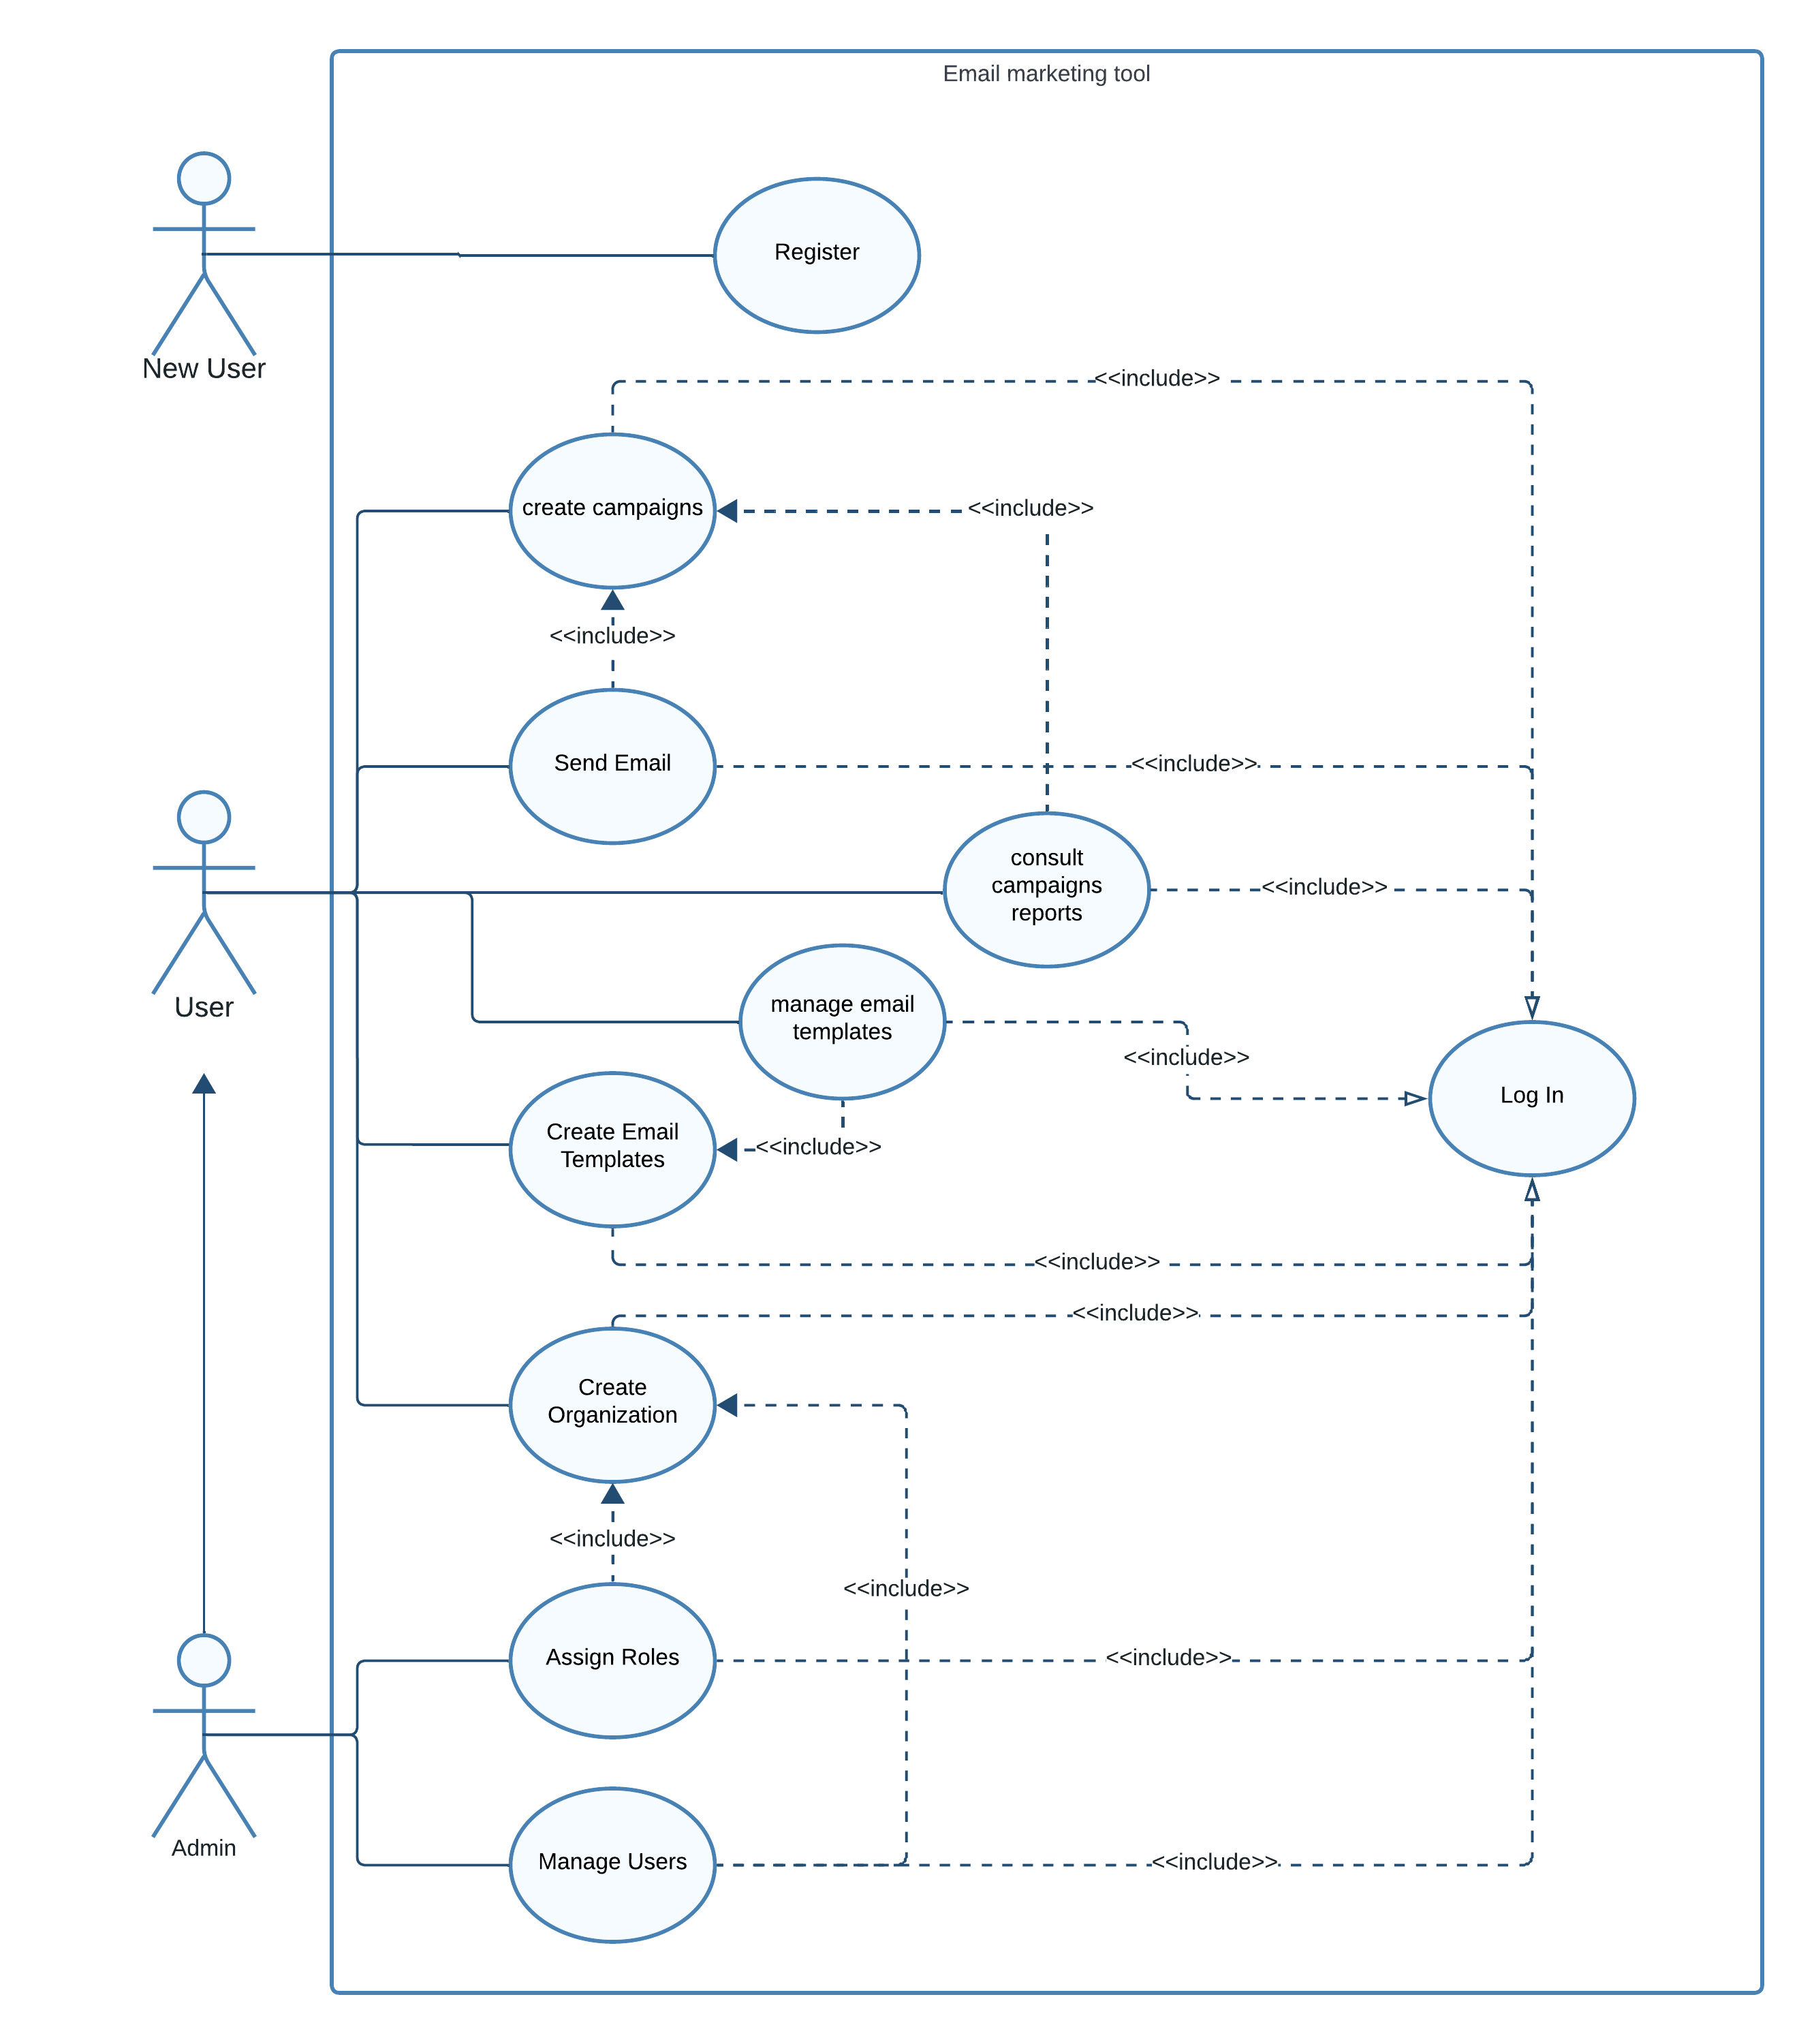
\includegraphics[width=\linewidth]{Images//images/global use case diag.png}
	\caption{Global Use Case Diagram}
	\label{fig:Global Use Case Diagram}
\end{figure}

\newpage

\subsection{Sprint Planning}

Figure \ref{fig:Sprint Planning} outlines our project's sprint planning. Each sprint had specific goals and durations. The initial phase was for learning the necessary tools. \textbf{Sprint 1} focused on building the email builder and creating and managing campaigns and audience. \textbf{Sprint 2} worked on media and organization management. \textbf{Sprint 3} focused on the deployment process and tracking functionality. This structured approach ensured thorough development and implementation of each feature. As a result, all planned features were successfully implemented within the project timeline.

\begin{figure}[ht]
    \centering
    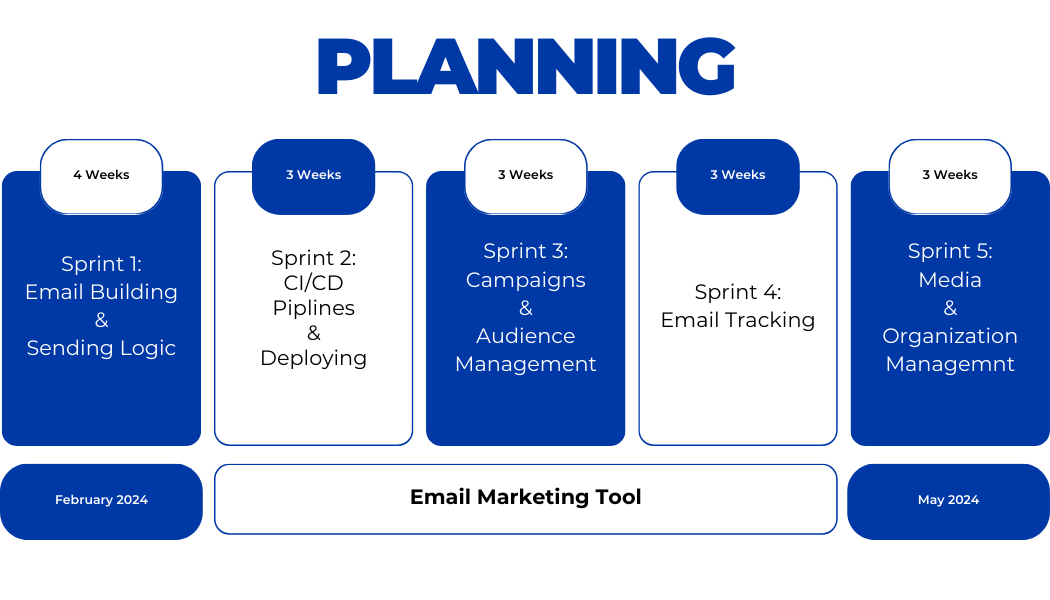
\includegraphics[width=\linewidth]{Images//images/planning.png}
    \caption{Sprint Planning}
    \label{fig:Sprint Planning}
\end{figure}


